\section{Auswertung}
\label{sec:Auswertung}

\subsection{Bestimmung der Apparaturwerte}

Zunächst muss die Winkelrichtgröße $D_\text{stat}$ der Spiralfeder bestimmt werden.
Hierzu wird die Formel
\begin{equation}
  D_\text{stat} = \frac{F \cdot r}{\varphi}
\end{equation}
mit den gemittelten Werten aus Tabelle \ref{tab:1} bemüht, wobei $r$ der Abstand zwischen Drehachse und anliegender Kraft, $\varphi$ der Auslenkwinkel und $F$ die anliegende Kraft ist.

\begin{table}[H]
  \centering
  \caption{Messdaten zur Bestimmung der Winkelrichtgröße.}
  \label{tab:1}
  \sisetup{table-format=1.2}
  \begin{tabular}{c c c c}
    \toprule
    {$r \ /\ 10^{-2}\si{\metre}$} & {$\varphi \ /\ \pi$} & {$F \ /\ \si{\newton}$} & {$D \ /\ 10^{-2}\si{\newton\metre}$}\\
    \midrule
    \input{build/statischtabelle.tex}
    \bottomrule
  \end{tabular}
\end{table}

Der sich ergebende gemittelte Wert für die Winkelrichtgröße lautet demnach
\begin{align*}
  D_\text{stat}   &=   \input{build/winkelrichtgroesse.tex}.
\end{align*}
Hierbei werden die angegebenen Auslenkwinkel mithilfe der Formel
\begin{equation}
  \varphi_\text{rad} = \frac{2 \pi}{360} \varphi_\text{deg}
\end{equation}
in Bogenmaß umgerechnet.
Um das Eigenträgheitsmoment $I_{\text{D}}$ der Drillachse zu bestimmen, werden die aufgenommenen Umlaufzeiten $T$ quadratisch gegen den Abstand $r$ von Drehachse zu den jeweiligen Testmassen zum Quadrat aufgetragen.
Mittels linearer Regression wird der y-Achsenabschnitt $b$ bestimmt.
Die Ausgleichsrechnung wird dabei von SciPy in Python durchgeführt.
Es werden die in Kapitel \ref{sec:fehler} angegebenen Fehlerformeln verwendet.

\begin{figure}
  \centering
  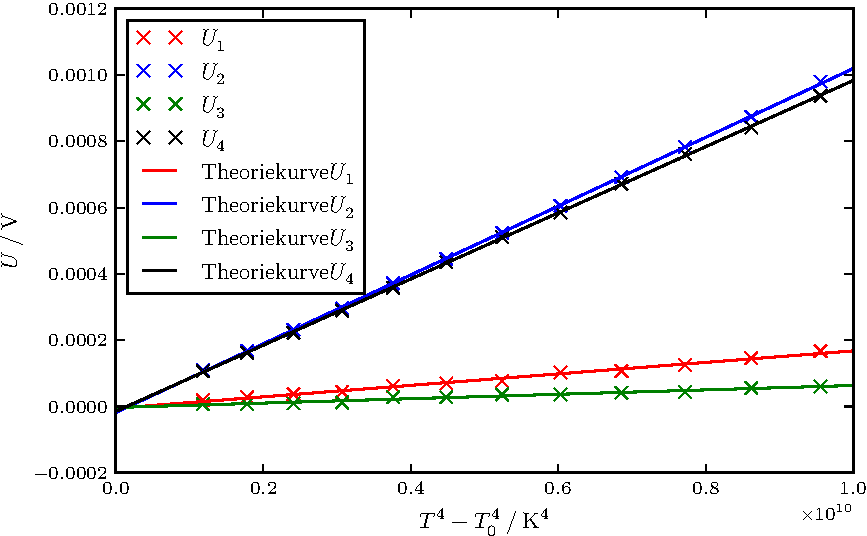
\includegraphics{plot.pdf}
  \caption{Plot zur Bestimmung des Eigenträgheitsmoments $I_{\text{D}}$ der Drillachse.}
  \label{fig:plot}
\end{figure}

Da die Zylindermassen als Punktmassen angenommen werden, ergibt sich aus dem Zusammenhang \eqref{eqn:tm1} für das Gesamtträgheitsmoment
\begin{equation}
  I_{\text{ges}} = I_{\text{D}} + (m_1+m_2)a².
\end{equation}
Hieraus folgt mit \eqref{eqn:zeiten} für die Quadrate der Umlaufzeiten
\begin{equation}
  T² = 4\pi² \frac{(m_1+m_2)}{D}r² + 4\pi² \frac{I_{\text{D}}}{D}.
\end{equation}
Folglich gilt für den aus der linearen Regression bestimmten Wert $b$,
\begin{align*}
  b = \input{build/b.tex},
\end{align*}
die Gleichung
\begin{equation}
  b = 4\pi² \frac{I_{\text{D}}}{D}
\end{equation}
und entsprechend
\begin{equation}
  I_{\text{D}} = \frac{b \cdot D}{4\pi²}.
\end{equation}
Daraus lässt sich nun die Eigenträgheit zu
\begin{align*}
  I_{\text{D}} = \input{build/eigentraegheit.tex}
\end{align*}
bestimmen.
Außerdem wird die Steigung der linearen Regression zu
\begin{align*}
  m_{\text{fit}} = \input{build/m.tex},
\end{align*}
bestimmt.
Hieraus lässt sich mithilfe der Beziehung
\begin{equation}
  D_\text{dyn} = \frac{4 \pi^2 (m_1 + m_2)}{m_\text{fit}}
\end{equation}
sowie der gemessenen Zylindermassen
\begin{align*}
m_1 &= \input{build/masse1.tex}\\
m_2 &= \input{build/masse2.tex}
\end{align*}
die dynamische Winkelrichtgröße zu
\begin{align*}
  D_\text{dyn}   &=   \input{build/winkelrichtgroesse_dyn.tex}.
\end{align*}
bestimmen.
\subsection{Bestimmung des Trägheitsmomentes eines Zylinders}
Die Durchführung der angegebenen Messreihen für den Zylinder führt zu den in Tabelle \ref{tab:zyl} angegebenen Werten

\begin{table}[H]
  \centering
  \caption{Messdaten zur Bestimmung des Trägheitsmomentes des Zylinders.}
  \label{tab:zyl}
  \sisetup{table-format=1.2}
  \begin{tabular}{c c c c}
    \toprule
    {$m_\text{zyl} \ /\ \si{\kilo\gram}$} & {$r_\text{zyl} \ /\ 10^{-2} \si{\metre}$} & {$h_\text{zyl} \ /\ 10^{-1}\si{\metre}$} & {$T_\text{zyl} \ /\ \si{\second}$}\\
    \midrule
    \input{build/zylindertabelle.tex}
    \bottomrule
  \end{tabular}
\end{table}

Aus diesen Messungen ergeben sich somit als Mittelwerte für die Eckdaten des Zylinders.
\begin{align*}
  R_{\text{Zylinder}} &= \input{build/r_zylinder.tex}, \\
  m_{\text{Zylinder}} &= \input{build/m_zylinder.tex}.
\end{align*}
Seine mittlere gemessene Umlaufzeit beträgt
\begin{align*}
  T_{\text{Zylinder}} = \input{build/t_zylinder.tex}
\end{align*}

Um sein theoretisches Trägheitsmoment zu bestimmen, wird die Formel für einen sich aufrechten drehenden Zylinder benutzt, welche
\begin{equation}
  I_{\text{Zylinder}} = \frac{mR²}{2}
\end{equation}
lautet.
Dementsprechend errechnet sich der theoretische Wert zu
\begin{align*}
  I_{\text{Zylinder, Theorie}} = \input{build/traegheit_zylinder_theorie.tex}. \\
\end{align*}

Aus der Gleichung (\ref{eqn:zeiten}) folgt der gemessene Wert des Trägheitsmomentes zu
\begin{align*}
  I_{\text{Zylinder, gemessen}} = \input{build/traegheit_zylinder.tex}.
\end{align*}
Dabei wird die Eigenträgheit $I_\text{D}$ nicht, wie theoretisch nötig, abgezogen.
Gründe hierfür werden in der Diskussion angegeben.
Zum Theoriewert ist eine relative Abweichung nach
\begin{equation}
  \increment I = \frac{I_{\text{Zylinder, gemessen}} - I_{\text{Zylinder, Theorie}}}{I_{\text{Zylinder, Theorie}}} \cdot 100
\end{equation}
von
\begin{align*}
  \increment I = \input{build/abweichung_zylinder.tex} \:\si{\percent} \\
\end{align*}
zu erkennen.


\subsection{Bestimmung des Trägheitsmomentes einer Kugel}
Für die Kugel werden die in Tabelle \ref{tab:kug} angegebenen Werte aufgenommen.

\begin{table}[H]
  \centering
  \caption{Messdaten zur Bestimmung des Trägheitsmomentes der Kugel.}
  \label{tab:kug}
  \sisetup{table-format=1.2}
  \begin{tabular}{c c c}
    \toprule
    {$m_\text{kug} \ /\ 10^{-1} \si{\kilo\gram}$} & {$d_\text{kug} \ /\ 10^{-1} \si{\metre}$} & {$T_\text{kug} \ /\ \si{\second}$}\\
    \midrule
    \input{build/kugeltabelle.tex}
    \bottomrule
  \end{tabular}
\end{table}

Die verwendete Kugel wird somit auf die Größen
\begin{align*}
  R_{\text{Kugel}} &= \input{build/r_kugel.tex}, \\
  m_{\text{Kugel}} &= \input{build/m_kugel.tex}
\end{align*}
vermessen, wobei ihre gemessene Umlaufzeit etwa
\begin{align*}
  T_{\text{Kugel}} = \input{build/t_kugel.tex}
\end{align*}
beträgt.
Es ergeben sich somit analog zur vorherigen Rechnung, jedoch mit einem Theorieträgheitsmoment für eine Kugel nach
\begin{equation}
  I_{\text{Kugel}} = \frac{2mR²}{5},
\end{equation}
die gemessenen und errechneten Trägheitsmomente
\begin{align*}
  I_{\text{Kugel, Theorie}}  &= \input{build/traegheit_kugel_theorie.tex} \\
  I_{\text{Kugel, gemessen}} &= \input{build/traegheit_kugel.tex}. \\
\end{align*}
Bei jener Kugel zeichnet sich eine relative Abweichung von
\begin{align*}
  \increment I = \input{build/abweichung_kugel.tex} \:\si{\percent}\\
\end{align*}
ab.


\subsection{Bestimmung des Trägheitsmomentes einer Puppe abhängig von ihrer Pose}
Zunächst werden in mehreren Messungen Eckdaten der verschiedenen Körperteile der Holzpuppe aufgenommen.
Die gemessenen Werte werden in den Tabellen \ref{tab:mensch}, \ref{tab:mensch2} und \ref{tab:mensch3} angegeben.

\begin{table}[H]
  \centering
  \caption{Messdaten zur Bestimmung des Trägheitsmomentes der Holzpuppe.}
  \label{tab:mensch}
  \sisetup{table-format=1.2}
  \begin{tabular}{c c c c c}
    \toprule
    {$m_\text{pup} \ /\ 10^{-1} \si{\kilo\gram} $} & {$h_\text{bein,1} \ /\ 10^{-1} \si{\metre}$} & {$h_\text{bein,2} 10^{-1} \ /\  \si{\metre}$} & {$d_\text{bein} \ /\ 10^{-2} \si{\metre}$} & {$a_\text{bein} \ /\ 10^{-2} \si{\metre}$}  \\
    \midrule
    \input{build/menschtabelle1.tex}
    \bottomrule
  \end{tabular}
\end{table}
Hierbei beschreibt $h_\text{bein,1}$ die Höhe des linken bzw. rechten Beins, $d_\text{bein}$ den Durchmesser der einzelnen Beine, $a_\text{bein}$ den Abstand der Mittelachsen der Beine voneinander.

\begin{table}[H]
  \centering
  \caption{Messdaten zur Bestimmung des Trägheitsmomentes der Holzpuppe.}
  \label{tab:mensch2}
  \sisetup{table-format=1.2}
  \begin{tabular}{c c c c c}
    \toprule
    {$h_\text{kopf} \ /\ 10^{-2} \si{\metre}$} & {$d_\text{kopf} \ /\ 10^{-2} \si{\metre}$} & {$h_\text{torso} \ /\ 10^{-2} \si{\metre}$} & {$d_\text{torso} \ /\ 10^{-2} \si{\metre}$} & {$l_\text{arme} \ /\ 10^{-1} \si{\metre}$}  \\
    \midrule
    \input{build/menschtabelle2.tex}
    \bottomrule
  \end{tabular}
\end{table}
\begin{table}[H]
  \centering
  \caption{Messdaten zur Bestimmung des Trägheitsmomentes der Holzpuppe.}
  \label{tab:mensch3}
  \sisetup{table-format=1.2}
  \begin{tabular}{c c c c}
    \toprule
    {$d_\text{arme} \ /\ 10^{-3} \si{\metre}$} & {$a_\text{arme} \ /\ 10^{-3} \si{\metre}$} & {$T_{\text{Pose1}} \ /\ 10^{-1} \si{\second}$} & {$T_{\text{Pose2}} \ /\ 10^{-1} \si{\second}$}  \\
    \midrule
    \input{build/menschtabelle3.tex}
    \bottomrule
  \end{tabular}
\end{table}

Hierbei beschreibt $h_\text{kopf}$ die Höhe des Kopfes, $d_\text{kopf}$ dessen Durchmesser, $h_\text{torso}$ die Höhe des Torsos, $d_\text{torso}$ dessen Durchmesser, $l_\text{arme}$ die Länge der Arme sowie $d_\text{arme}$ dessen Durchmesser und $a_\text{arme}$ den Abstand der Mittelachsen der Arme in anliegender Pose voneinander.

Die gemittelten Maße der benutzten Holzpuppe betragen somit
\begin{align*}
  L_{\text{Bein1}}  &= \input{build/laenge_b_1.tex}, \\
  L_{\text{Bein2}}  &= \input{build/laenge_b_2.tex}, \\
  R_{\text{Beine}}   &= \input{build/radius_b.tex}, \\
  a_{\text{Beine}}   &= \input{build/abstand_b.tex}, \\
  L_{\text{Torso}}   &= \input{build/laenge_t.tex}, \\
  R_{\text{Torso}}   &= \input{build/radius_t.tex}, \\
  L_{\text{Kopf}}    &= \input{build/laenge_k.tex}, \\
  R_{\text{Kopf}}    &= \input{build/radius_k.tex}, \\
  L_{\text{Arme}}    &= \input{build/laenge_a.tex}, \\
  R_{\text{Arme}}    &= \input{build/radius_a.tex}, \\
  a_{\text{Arme}}    &= \input{build/abstand_a.tex}, \\
  m_{\text{ges}}     &= \input{build/masse.tex} \\
\end{align*}
wobei $L$ für Länge, $R$ für Radius, $a$ für den Abstand zur Drehachse und $m$ für die Gesamtmasse steht.
Aus diesen Daten folgt für die Volumina der einzelnen approximierten Körperteile
\begin{align*}
  V_{\text{Arm1}}  &= \input{build/volumen_arm_1.tex}, \\
  %V_{\text{Arm2}}  &= \input{build/volumen_arm_2.tex}, \\
  V_{\text{Bein1}}  &= \input{build/volumen_bein_1.tex}, \\
  V_{\text{Bein2}}  &= \input{build/volumen_bein_2.tex}, \\
  V_{\text{Kopf}}  &= \input{build/volumen_kopf.tex}, \\
  V_{\text{Torso}}  &= \input{build/volumen_torso.tex}, \\
\end{align*}
Die Dichte der Holzpuppe errechnet sich aus dem Gesamtvolumen
\begin{align*}
  V_\text{Ges} &= \input{build/volumen_mensch.tex},
\end{align*}
und der oben angegebenen Gesamtmasse zu
\begin{align*}
  \rho &= \input{build/dichte_mensch.tex}.
\end{align*}
Hieraus folgen dementsprechend die einzelnen Massen der Körperteile zu
\begin{align*}
  m_{\text{Arm1}}  &= \input{build/masse_arm_1.tex}, \\
  %V_{\text{Arm2}}  &= \input{build/volumen_arm_2.tex}, \\
  m_{\text{Bein1}}  &= \input{build/masse_bein_1.tex}, \\
  m_{\text{Bein2}}  &= \input{build/masse_bein_2.tex}, \\
  m_{\text{Kopf}}  &= \input{build/masse_kopf.tex}, \\
  m_{\text{Torso}}  &= \input{build/masse_torso.tex}.
\end{align*}
Im Weiteren folgen für die Trägheitsmomente der einzelnen Körperteile
\begin{align*}
  I_{\text{Arm, Pose1}}  &= \input{build/traegheit_arm_pose1.tex}, \\
  I_{\text{Arm, Pose2}}  &= \input{build/traegheit_arm_pose2.tex}, \\
  I_{\text{Bein1}}  &= \input{build/traegheit_bein_1.tex}, \\
  I_{\text{Bein2}}  &= \input{build/traegheit_bein_2.tex}, \\
  I_{\text{Kopf}}  &= \input{build/traegheit_kopf.tex}, \\
  I_{\text{Torso}}  &= \input{build/traegheit_torso.tex},
\end{align*}
wobei es sich hierbei um die Trägheitsmomente um die Symmetrieachse des jeweiligen Körpers handelt.
Nach Ergänzen der Formel für das Trägheitsmoment auf der Seite liegender Zylinder,
\begin{equation}
  I_{\text{Zylinder}} = m \left( \frac{R²}{4} + \frac{L²}{12} \right),
\end{equation}
folgt, unter Anwendung des Steinerschen Satzes, das theoretische Trägheitsmoment in der ersten Pose zu
\begin{align*}
  I_{\text{Theorie, Pose1}}  &= \input{build/traegheit_mensch_pose_1_theorie.tex}. \\
\end{align*}
Der gemessene Wert
\begin{align*}
  T_{\text{Pose1}}  &= \input{build/t1.tex} \\
\end{align*}
führt auf ein Trägheitsmoment von
\begin{align*}
  I_{\text{gemessen, Pose1}}  &= \input{build/traegheit_mensch_pose_1.tex}. \\
\end{align*}
Die hier vorliegende prozentuale Abweichung zum Theoriewert beträgt
\begin{align*}
  \increment I  &= \input{build/abweichung_pose_1.tex}\:\si{\percent}. \\
\end{align*}

Analog folgen die Werte zur zweiten Pose durch
\begin{align*}
  T_{\text{Pose2}}  &= \input{build/t2.tex} \\
\end{align*}
auf
\begin{align*}
  I_{\text{Theorie, Pose2}}   &= \input{build/traegheit_mensch_pose_2_theorie.tex}, \\
  I_{\text{gemessen, Pose2}}  &= \input{build/traegheit_mensch_pose_2.tex}, \\
  \increment I                 &= \input{build/abweichung_pose_2.tex}\:\si{\percent}. \\
\end{align*}




%\subsection{Bestimmung des Trägheitsmomentes einer Puppe abhängig von ihrer Pose}
%Die gemittelten Maße der benutzten Holzpuppe betragen
%\begin{align*}
%  L_{\text{Bein_1}}  &= \input{build/laenge_b_1.tex}, \\
%  L_{\text{Bein_2}}  &= \input{build/laenge_b_2.tex}, \\
%  R_{\text{Beine}}   &= \input{build/radius_b.tex}, \\
%  a_{\text{Beine}}   &= \input{build/abstand_b.tex}, \\
%  L_{\text{Torso}}   &= \input{build/laenge_t.tex}, \\
%  R_{\text{Torso}}   &= \input{build/radius_t.tex}, \\
%  L_{\text{Kopf}}    &= \input{build/laenge_k.tex}, \\
%  R_{\text{Kopf}}    &= \input{build/radius_k.tex}, \\
%  L_{\text{Arme}}    &= \input{build/laenge_a.tex}, \\
%  R_{\text{Arme}}    &= \input{build/radius_a.tex}, \\
%  a_{\text{Arme}}    &= \input{build/abstand_a.tex}, \\
%  m_{\text{ges}}     &= \input{build/masse.tex} \\
%\end{align*}
%wobei $L$ für Länge, $R$ für Radius, $a$ für den Abstand zur Drehachse und $m$ für die Gesamtmasse steht.
%Nach ergänzen der Formel für das Trägheitsmoment auf der Seite liegender Zylinder,
%\begin{equation}
%  I_{\text{Zylinder}} = m \left( \frac{R²}{4} + \frac{L²}{12} \right),
%\end{equation}
%
%folgt das theoretische Trägheitsmoment in der ersten Pose zu
%\begin{align*}
%  I_{\text{Theorie, Pose_1}}  &= \input{build/traegheit_mensch_pose_1_theorie.tex}. \\
%\end{align*}
%Der gemessene Wert
%\begin{align*}
%  T_{\text{Pose_1}}  &= \input{build/t1.tex} \\
%\end{align*}
%führt auf ein Trägheitsmoment von
%\begin{align*}
%  I_{\text{gemessen, Pose_1}}  &= \input{build/traegheit_mensch_pose_1.tex}. \\
%\end{align*}
%Die hier vorliegende prozentuale Abweichung zum Theoriewert beträgt
%\begin{align*}
%  \increment I  &= \input{build/abweichung_pose_1.tex}\:\si{\percent}. \\
%\end{align*}
%
%Analog folgen die Werte zur zweiten Pose durch
%\begin{align*}
%  T_{\text{Pose_2}}  &= \input{build/t2.tex} \\
%\end{align*}
%auf
%\begin{align*}
%  I_{\text{Theorie, Pose_2}}   &= \input{build/traegheit_mensch_pose_2_theorie.tex}, \\
%  I_{\text{gemessen, Pose_2}}  &= \input{build/traegheit_mensch_pose_2.tex}, \\
%  \increment I                 &= \input{build/abweichung_pose_1.tex}\:\si{\percent}. \\
%\end{align*}


%\begin{figure}
%  \centering
%  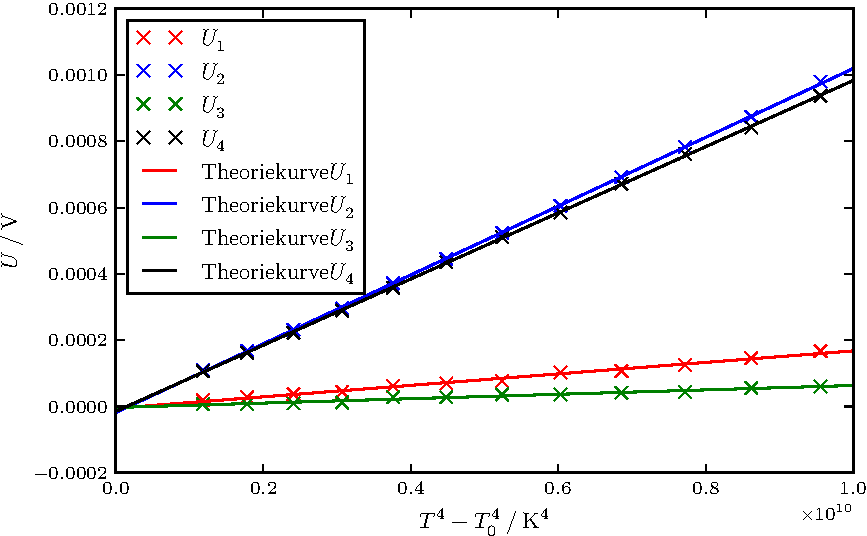
\includegraphics{plot.pdf}
%  \caption{Plot.}
%  \label{fig:plot}
%\end{figure}
%
%\begin{table}
%  \centering
%  \caption{Beispieltabelle}
%  \label{tab:tabelle_beispiel}
%  \sisetup{table-format=1.2}
%  \begin{tabular}{c c}
%    \toprule
%    {$a [\si{\second}]$} & {$b [\si{\kelvin}]$}\\
%    \midrule
%    1.0000  & 11.00 \\
2.0000  & 12.00 \\
3.0000  & 13.00 \\
4.0000  & 14.00 \\
5.0000  & 15.00 \\
6.0000  & 16.00 \\
7.0000  & 17.00 \\
8.0000  & 18.00 \\
9.0000  & 19.00 \\
10.0000 & 20.00 \\

%    \bottomrule
%  \end{tabular}
%\end{table}
%
%Es ergibt sich
%\begin{align}
%  a &= (0 \pm 0) ~ \si{\joule\per\kelvin\per\gram}
 \\
%\end{align}
%
